\documentclass[border=5mm]{standalone}
\usepackage{tikz}
\usetikzlibrary{fadings}
\tikzfading[name=fade right,
left color=transparent!0,
right color=transparent!100]
\tikzfading[name=fade left,
left color=transparent!100,
right color=transparent!0]
\begin{document}
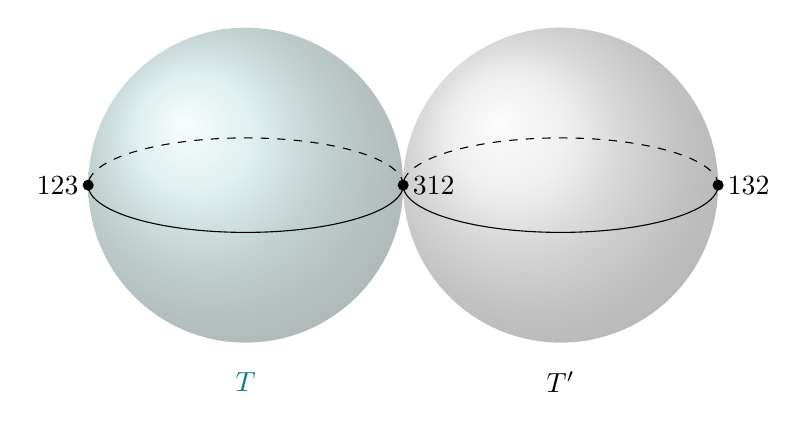
\begin{tikzpicture}
  \shade[ball color = teal!40, opacity = 0.4] (8,0) circle (2cm);
  \shade[ball color = gray!40, opacity = 0.4] (12,0) circle (2cm);
  \fill[fill=black] (6,0) circle (2pt);
  \node[left] at (6,0) {123};
  \draw (6,0) arc (180:360:2 and 0.6);
  \draw[dashed] (10,0) arc (0:180:2 and 0.6);
  \fill[fill=black] (10,0) circle (2pt);
  \draw (10,0) arc (180:360:2 and 0.6);
  \draw[dashed] (14,0) arc (0:180:2 and 0.6);
  \fill[fill=black] (14,0) circle (2pt);
  \node[right] at (14,0) {132};
  \node[right] at (10,0) {312};
  \node[] at (8,-2.5) {\color{teal}$T$};
  \node[] at (12,-2.5) {$T'$};
\end{tikzpicture}
\end{document}
